\chapter{Conclusion}
\label{conclusion}
This chapter describes the final system that was created through the project. This includes two native applications and a \gls{backend} solution that provides a \gls{REST}ful \gls{API}. Because it was created using a specialized development process to comply with the \gls{LSU}-methodology, this chapter will also describe the finalized structure of that process. Section \ref{ios-conclusion} describes the finalized iOS application, section \ref{android-conclusion} describes the final Android application, while section \ref{backend-conclusion} describes the final \gls{backend} solution.


\section{Development process}
The development process used in this project was based in the \gls{LSU} methodology and includes some features from Scrum. A generic example is described in section \ref{generic-example}. Following the build-measure-learn feedback loop, illustrated in figure \ref{fig:build-measure-learn}, the iteration begins creating an assumption about the users that needs to be confirmed. To learn the truth about the assumption the team discuss possible alternatives and creates user stories as backlog to be implemented, derived from Scrum. The product is created in a manner that makes it easy to measure the validity of the assumption. After measuring the use of the product the team will know the validity of the assumption and select to  either continue with that idea or try something else. At the end of the version the team will have a review meeting with the customer to show the result and a retrospective meeting to discuss the team process. These meetings are also derived from the Scrum methodology.


\section{System overview}
\label{conclusion-system-overview}
The complete system consists of a server application which talks to database system MongoDB. There are two client applications, one for Android and one for iOS. Each of these use the Google Books \gls{API} to fetch meta information about books. See figure \ref{fig:system-arch-final-simple} in chapter \ref{chap:ArchitecturalDescription}. 

\subsection{The iOS application overview}
\label{ios-conclusion}
The iOS application has come a long way during this project. It has evolved from a crude prototype to a full-fledged application. This process is described in chapter \ref{chap:LeanStartup}. This section provides an overview of the final version.

Save for a few bugs, the application is now fully functional and satisfies all  requirements defined in section \ref{requirements}. The architecture by which it achieves this is defined in section \ref{architecture-ios} in the architectural description.

Figure \ref{fig:navigation-tree-ios-6} illustrates the final design, and how the various views are connected.

\begin{figure}
    \begin{center}
        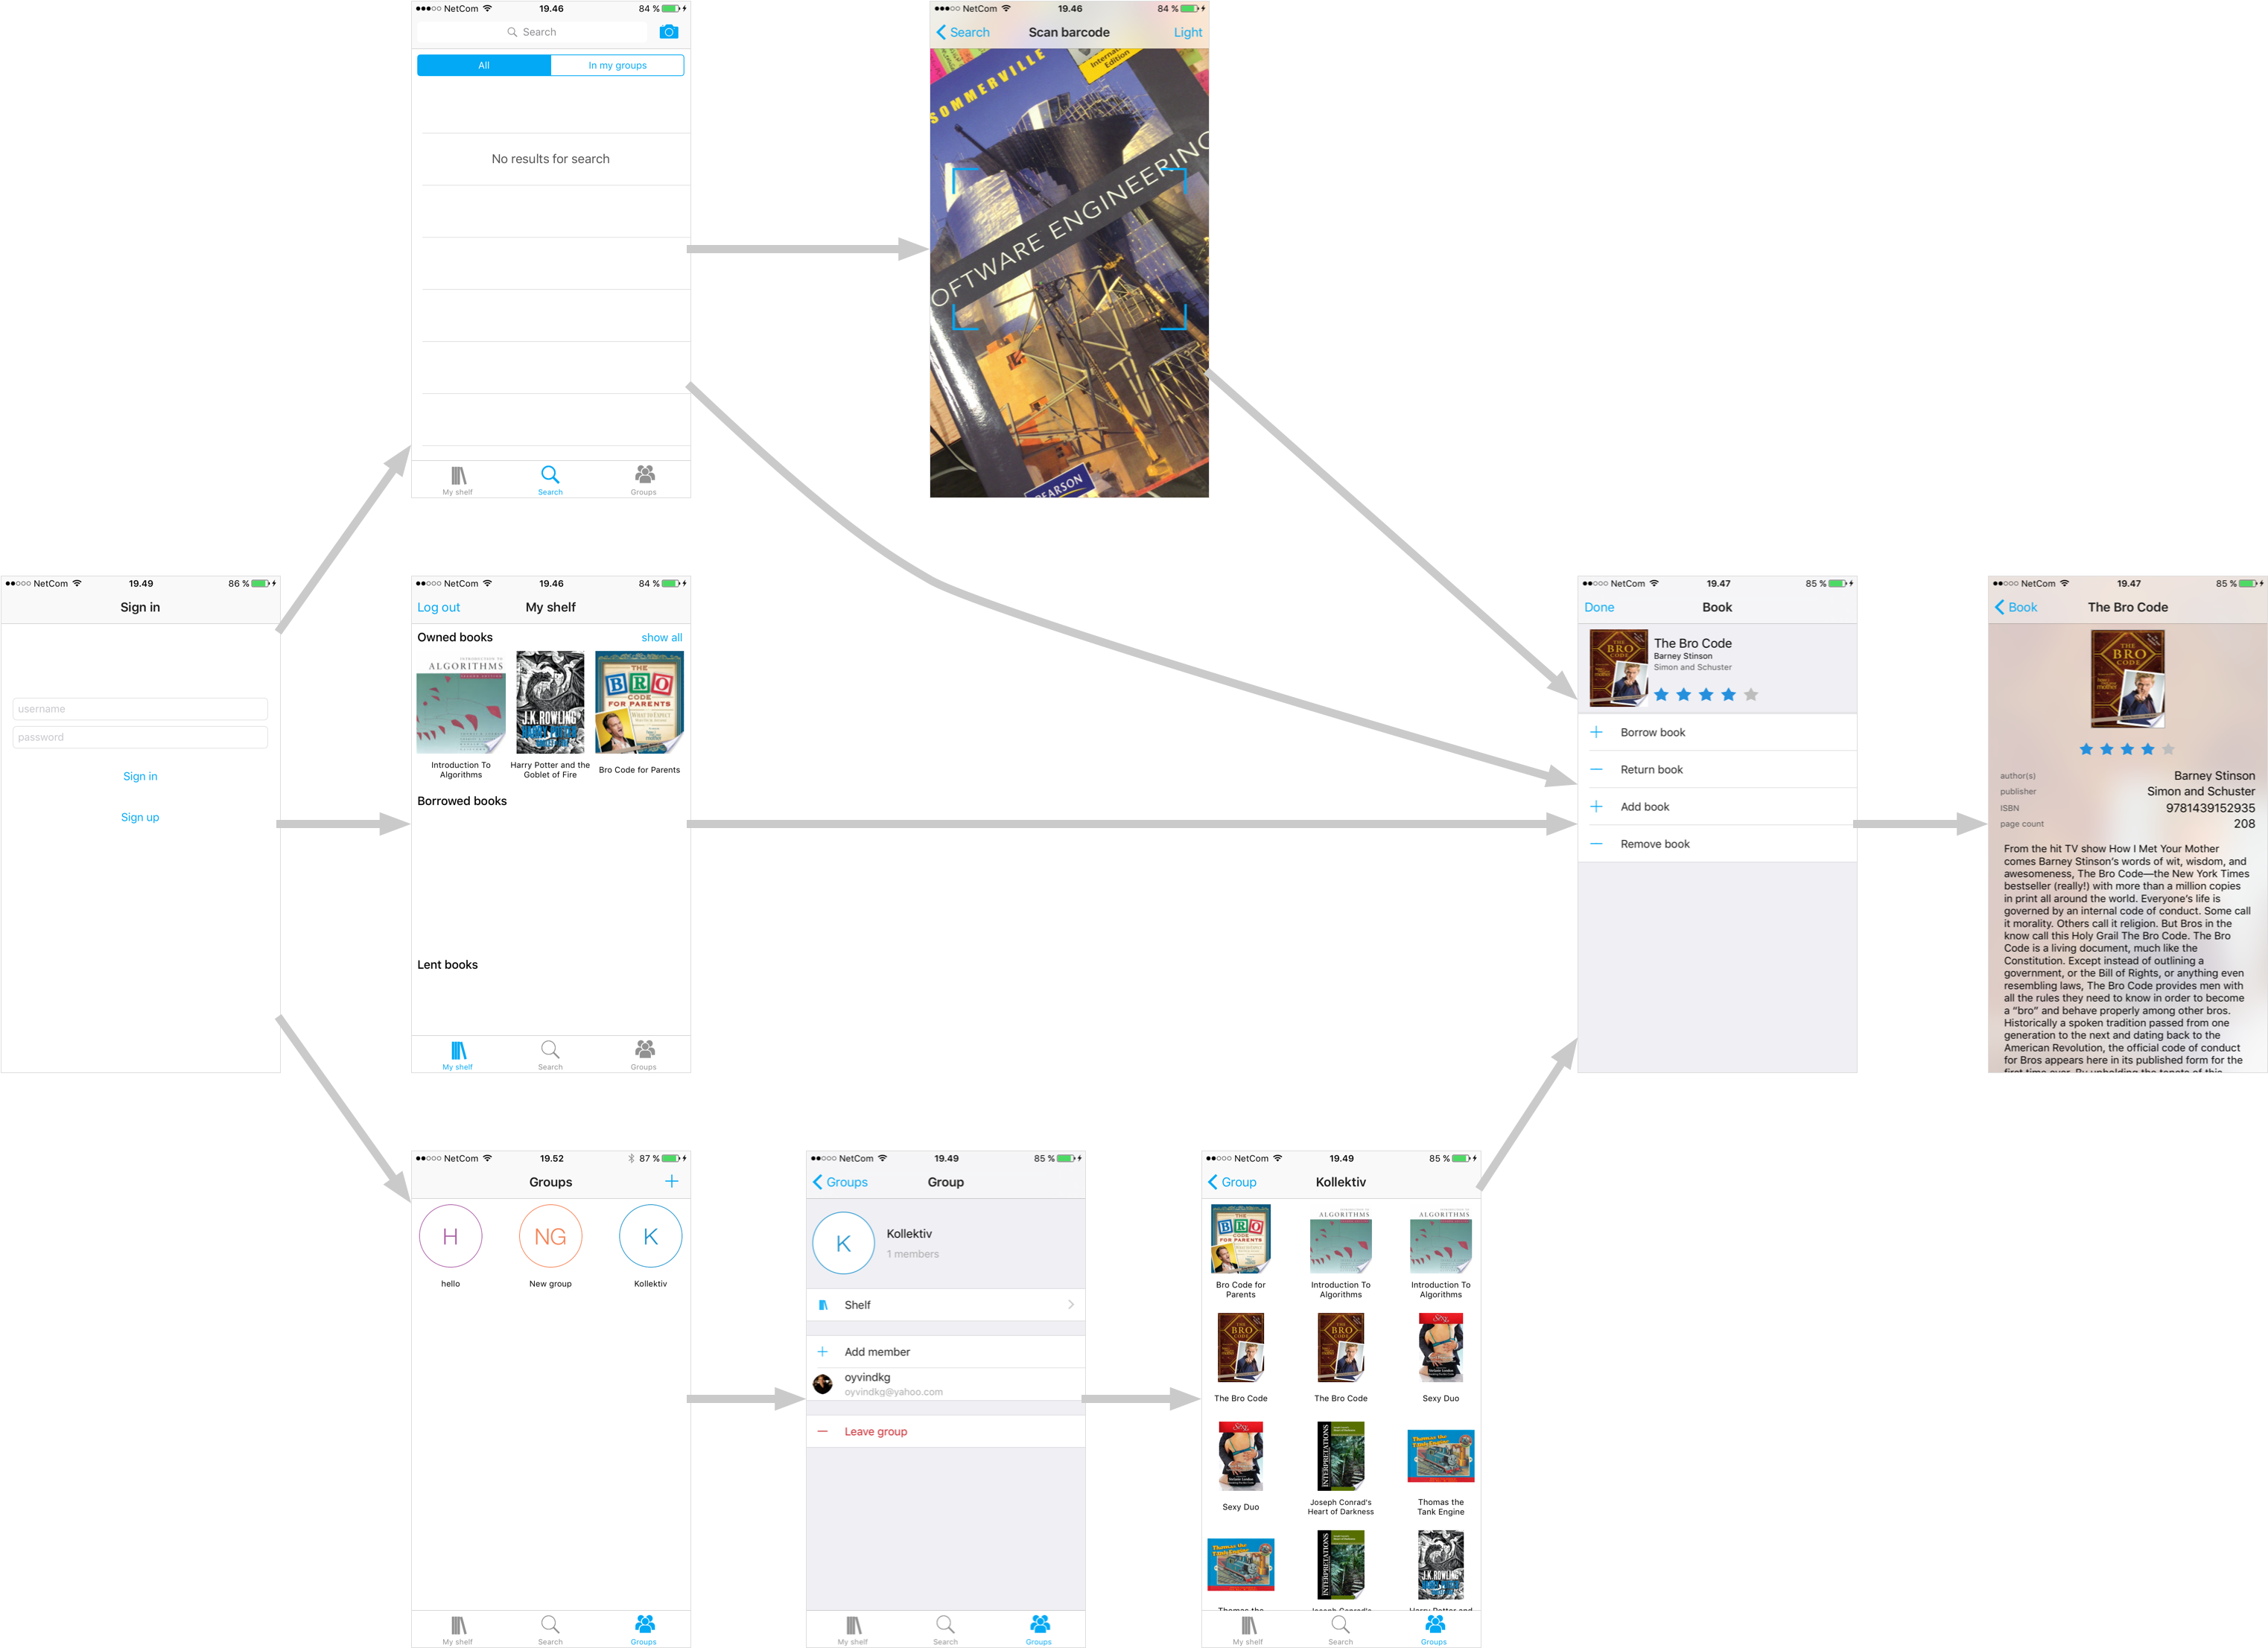
\includegraphics[width=\textwidth,keepaspectratio]{figs/v06/iOS/navigation-tree-ios.png}
        \caption{A diagram showing the final design of the iOS application.}
        \label{fig:navigation-tree-ios-6}
    \end{center}
\end{figure}



\subsection{The Android application overview}
\label{android-conclusion}
The Android application started out as a simple non-user friendly designed application, and has by user feedback and experience evolved into a working application. This section provides an overview of the final version of the application that can be seen in figure \ref{fig:AndroidFinalDesign}. 

The final version of the Android application satisfies all requirements defined in section \ref{requirements}. The application implements both social and user friendly features such as the possibility to borrow books from other users in groups, and the ability to add a book to the user's book shelf using the camera of the device. The design of the application has evolved greatly over the course of the different version as can be seen in figure \ref{fig:AndroidBookView05}. The current design of the application and how the different views interact can be seen in figure \ref{fig:AndroidFinalDesign}. The architecture used to implement this application is described in detail in section \ref{architecture-android}.



\begin{figure}
    \begin{center}
        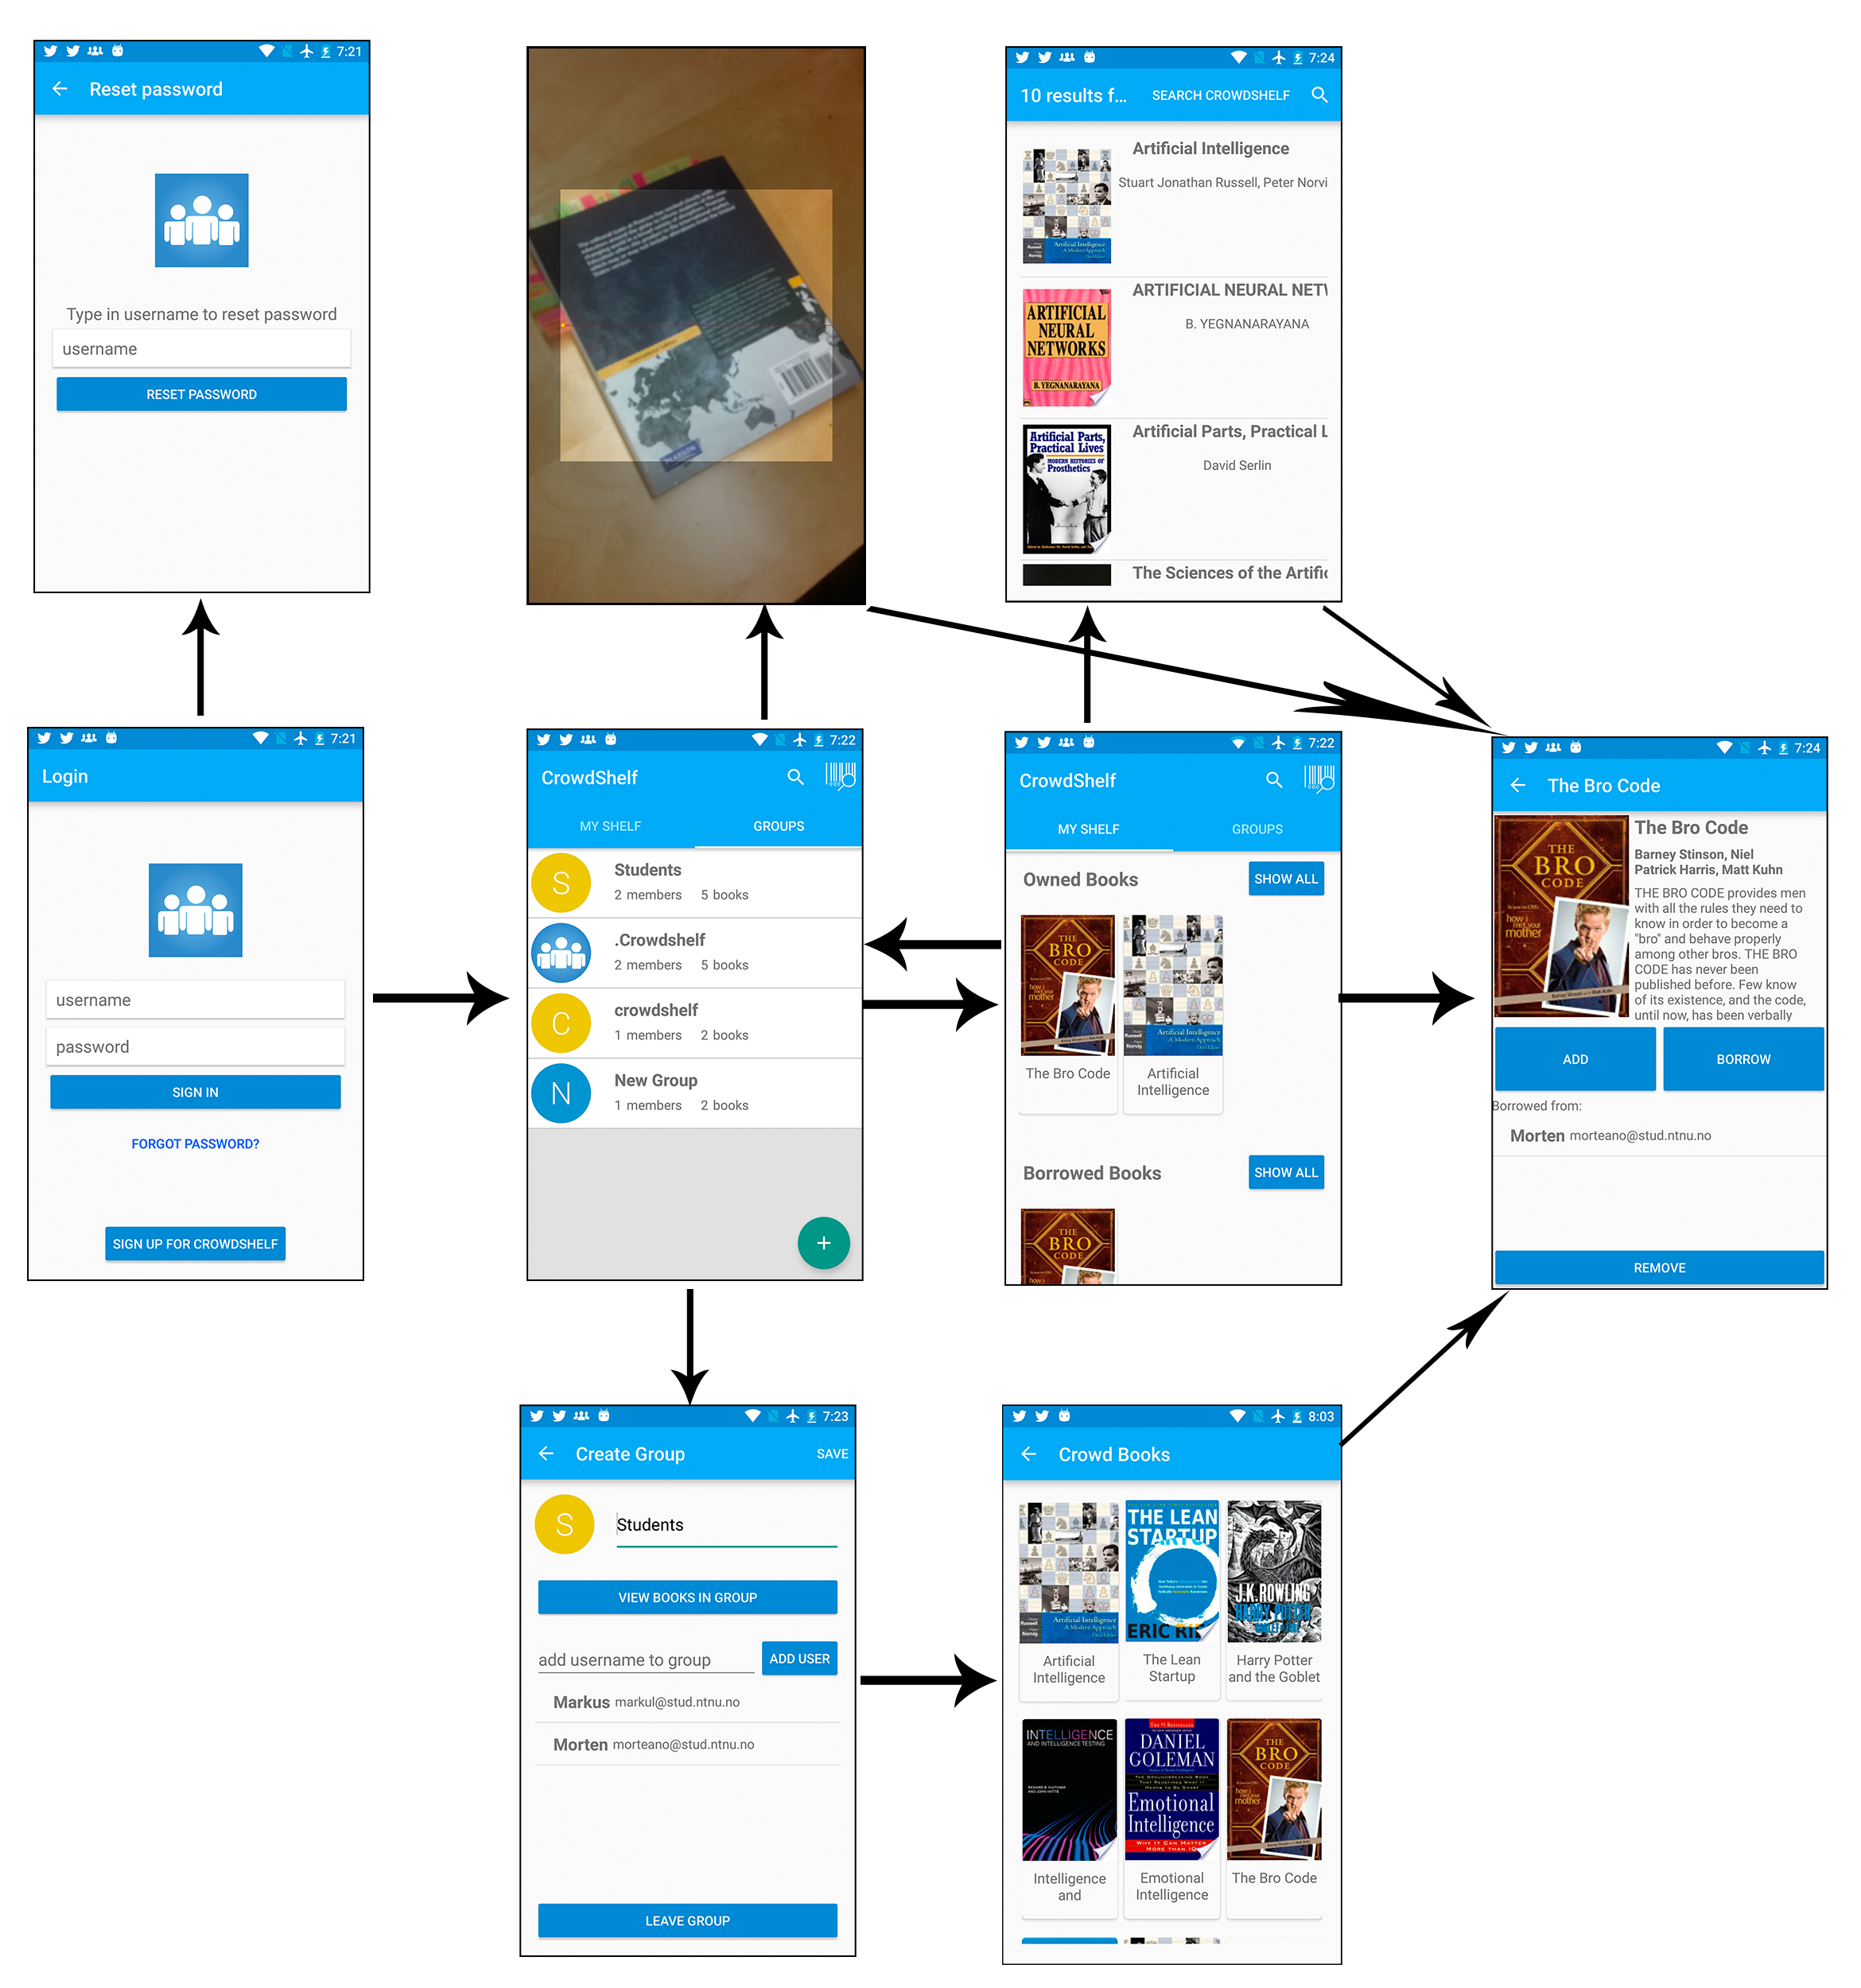
\includegraphics[width=.5\textwidth,keepaspectratio]{figs/AndroidFinalDesign.png}
        \caption{A diagram showing the final design of the Android application.}
        \label{fig:AndroidFinalDesign}
    \end{center}
\end{figure}




\section{Backend overview}
\label{backend-conclusion}
The team developed a server application that talks to a MongoDB database system. The server application itself is written in Node with the Express framework. It is oriented around a set of modules, that are structured into \code{controllers}, \code{models} and \code{helpers}. The overall structure of the application can be seen in figure \ref{fig:server-detail}. The code is available on GitHub. There is written a so called ''dockerfile'', that can be used to build a Docker-image. The team set up the Docker Hub to pull changes from \code{master}-\gls{branch} on GitHub, and automatically build a new image. The team set up a server on Digital Ocean, under the domain \url{crowdshelf.xyz}, that automatically pulls the image and restarts it when Docker Hub has rebuilt it.  \cite{docker}\cite{dockerhub-crowdshelf} There is also a development server that runs on Heroku, that pulls changes from the \code{dev}-\gls{branch} on GitHub, and redeploys that server application automatically under the domain \url{crowdshelf-dev.herokuapp.com}. For more information on deployment, see appendix \ref{app:backend-readme}, which is the developers documentation for the server project.

\section{Further work}
Although this project is complete there are a lot of possibilities for further work with both the applications and the \gls{API}. Both in the area of development and in getting more users of the application.


\subsection{Expand the area of use}
Early on, the customer representative mentioned a possible extension of the application. This was to let it support other objects than books. In this sense allow the users to share any items they wanted, and to keep them organized through one single application. 

If the application continues to use a barcode scanner to add items, everything with a barcode can potentially be borrowed as long as there is implemented some way to identify the items. Some items like DVDs, CDs, and computer games could be included with only minor changes, while if for instance tools should be added, it would need some improvement on the search function. This is because the items would then change from having a couple different barcodes, to hundreds or thousands.

All of the code written in this project is licensed under the MIT Licence (See Appendix \ref{app:license}) which  allows anyone to further develop or edit the code.  Hopefully the code will be reused and further developed so that the application can continue to be improved and to support the needs of the users.

In this project, the \gls{API} is created as a independent product. It is documented on Swagger so it will be easy to use for other developers. Anyone can easily combine the \gls{API}  with other systems if they for example want to create specialized applications. It is also possible to change parts of the \gls{API} or only use some of its functionality

\subsection{Increase the customer base}
Another angle of improving the application is to increase the number of customers. This would make it easier to learn about the users and design an application they desire. 

During this project the development team has already been in contact with some potential customers, and both Rosenholm primary school and the police station in Grønland, represented by district attorney Olav Helge Thue, are interested in the application.

A problem with having Norwegian customers is that Norwegian books are not always located in Google Books database. In this project it was an attempt to solve that problem by creating a book service so the users could save books. Even though it was not possible to develop that service in this project it is a feature that can give the application a larger customer base by providing a large variety of books.

Other potential customers are all companies that have a common book shelf. And observed in this project there are a few of them. 

\subsection{Creating a sustainable product}
If the customer base grows it might be necessary to consider how the operation of the application can be sustainable.
A suggestion to achieve this is to add ads to the applications. However this might not be a good alternative since all the code is MIT licensed. Anyone could  download the code, comment out the ads and publish the ad-free system as their own. 

Another possibility is to deploy paid versions of the application on Google Play and App store, but for this to be a valid option some features have to be added without the MIT licence.

The best alternative the group found is to link to an online bookstore, like Amazon, and get an advertising fee when users buy books from it. For instance, if a user searches for a book, but no one in the user's group owns the book, a message that links to Amazon could be displayed; "No user in your groups got this book. Go to \url{amazon.com} to buy the book".

